\chapter{Snapshot}
\label{chap:snapshot}

    One of the major features in Kabi File System is the writable copy-on-write snapshot. A snapshot is a point-in-time copy of a defined collection of data \cite{snapshot_def}. A read only snapshot is an immutable copy of the file system data at a time spot, while a writable snapshot can be considered as a writable fork of such copy. Snapshot nodes are designed as the basic components of Kabi File System. The ``current'' view of the file system is also treated as a writable snapshot (the latest snapshot in default branch). This snapshot system focuses on reducing the storage space occupied by a snapshot.

    According to the Storage Networking Industry Association, three classic snapshot approachs include split-mirror, changed block, and concurrent.\cite{snapshot_types} The split-mirror approach copies every byte from source to snapshot. The process is time consuming hence it usually requires planning in advance. The changed block approach applies copy-on-write on the snapshot. The concurrent approach redirects IO request to different storage spaces associated with snapshots. Instead of making a copy and overwrite the copy, write IO request will be redirected a seperate storage space. While a read IO request will be redirected depends on whether the data has been changed since last snapshot.

    Our snapshot system uses a stratergy that is a mixture of copy-on-write and redirect IO. It uses enhanced copy-on-write stratergy on actual data and Redirect IO stratergy on meta data. In our snapshot system, most snapshots do not keep a copy of the entire file system but instead log the changes since the last snapshot. Such that the snapshot system can then recover the content of the a snapshot based on the previous snapshot and the log of changes, as shown in \fref{fig:snapshot_patch} The only exception is a special snapshot called head snapshot which contains contents of the entire file system at a particular time. Other snapshots are called referencing snapshot. They contain a reference to another snapshot and an array of patch objects. Each patch object in the array reflects a series of changes on a single file or a single directory since the last snapshot.

\begin{figure}[t]
\centering
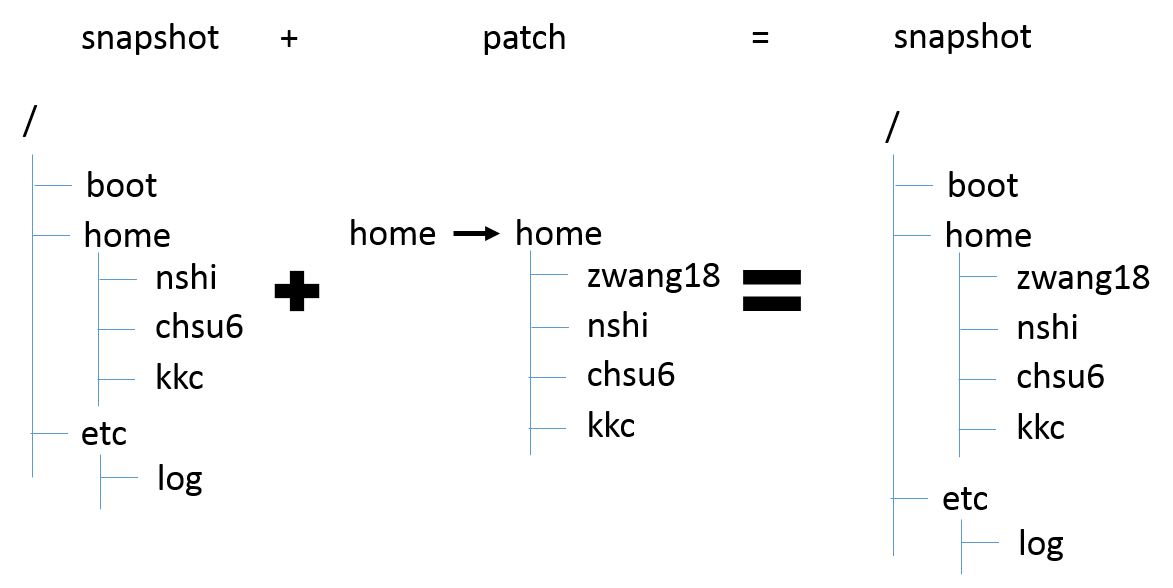
\includegraphics[width=0.8\textwidth]{Chapter-4/figs/fig23.png}
\caption{Snapshots and Patches}
\label{fig:snapshot_patch}
\end{figure}

\section{The Snapshot Tree}

	The snapshot system in Kabi File System uses a approach based on patches. Similar approach adpoted by ext3cow uses a reserved field in inode to reference the previous version inode shown in \fref{fig:snapfs_approach}. One advantage of the patch based approach is that it supports tree structured snapshots and writable snapshots.

\begin{figure}[t]
\centering
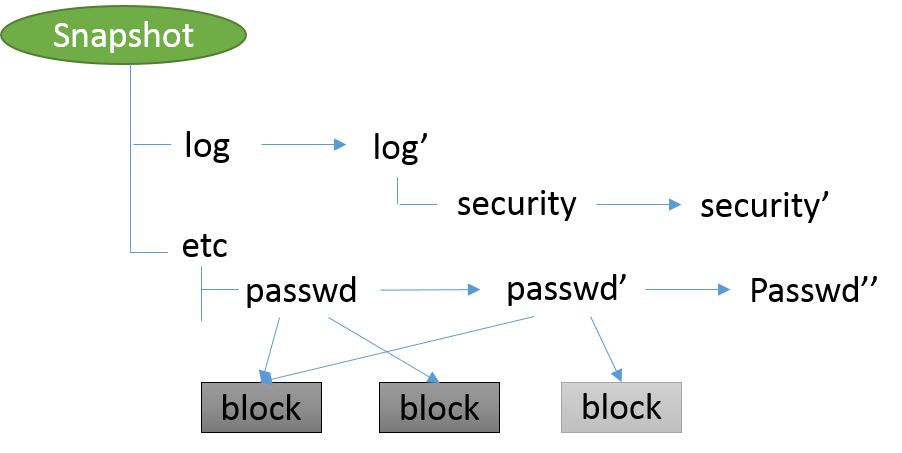
\includegraphics[width=0.7\textwidth]{Chapter-4/figs/fig24.png}
\caption{Snapshots in SnapFS}
\label{fig:snapfs_approach}
\end{figure}

    Snapshots in the Kabi File System are represented by snapshot node and forms an up-tree. In an up-tree, all child reference or point to its parent. The following \fref{fig:snap_tree_example} shows an example of the snapshot tree. The right bottom node (node 0) is the root of the tree. The root of the snapshot tree is always the head snapshot.

\begin{figure}[t]
\centering
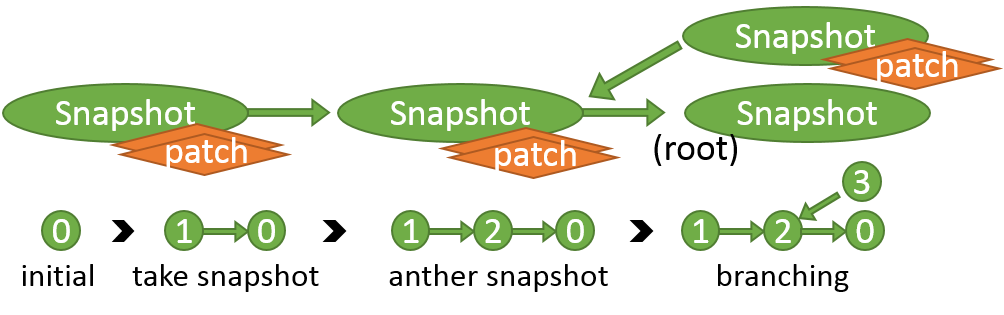
\includegraphics[width=0.8\textwidth]{Chapter-4/figs/fig13.png}
\caption{An example of snapshot tree}
\label{fig:snap_tree_example}
\end{figure}

    Initially, the file system contains a default writeable snapshot node (node 0 in \fref{fig:snap_tree_example}) representing the current view of the file system. This special snapshot called the head snapshot is the root of the snapshot tree and the only snapshot node that does not reference other snapshot. For initial state, any writes to the file system go directly into the head snapshot.
    
    After a snapshot is taken, a new snapshot node (node 1 in \fref{fig:snap_tree_example}) is created referring to the head snapshot node. Subsequent write operations will not only write data into the head snapshot but also submit patches to all snapshot connected to head snapshot, so as to reflect the difference between snapshot node 1 and its referencing node 0.

    Branching a snapshot creates a writable copy of a existing snapshot. The branching operation is implemented by creating a new snapshot node referring the snapshot being forked. As shown in \fref{fig:snap_tree_example}, node 3 (the writable copy) is created and connected to snapshot node 2 (the exisiting snapshot) in order to fork the file system based on snapshot 2.

    In the snapshot tree, each writable snapshot correspond to a branch. A branch consists of the writable snapshot (the current status of the branch) and its historical snapshots (the history of the branch). The main branch is the branch where the head snapshot node lies. \fref{fig:branches} shows the idea of branch. in the example, there are two branches in this 5-node snapshot tree. Node 0 is the root of the uptree so corresponds to the head snapshot. Thus node 1, node 2, and node 0 form the main branch. In the figure, nodes on the left corresponds to an older snapshot and nodes on the right corresponds to a more recent snapshot. Therefore in main branch, node 1 is the oldest snapshot while node 0 represents the latest state. Node 1 and Node 2 form the history of main branch and node 0 is the current view of main branch. Node 4 is another writable snapshot and it belongs to a side branch. The side branch consists of node 1 (the oldest), node 2 (the second oldest), node 3 (the third oldest), and node 4 (most recent). Note that arrows between nodes reflect the referencing relations between snapshots, not the order of creation.

\begin{figure}[t]
\centering
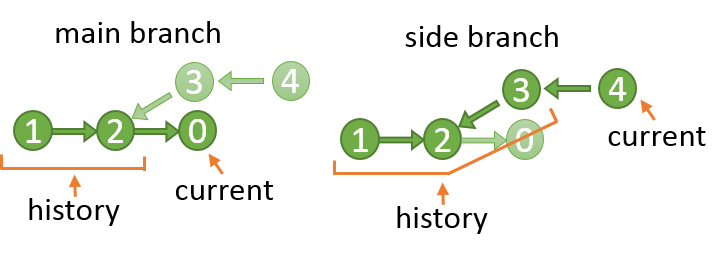
\includegraphics[width=0.65\textwidth]{Chapter-4/figs/fig22.png}
\caption{Branches}
\label{fig:branches}
\end{figure}

\section{Snapsho Nodes and Patch Object}

    As mentioned in previous section, there are two types of snapshot node in this file system, namely the head snapshot node and the referencing snapshot node.

    The head snapshot is special in the file system. It is the root of the up-tree and does not reference any other snapshots. Instead it stores the entire content of current view of main branch by referencing the directory node of the root directory. In this way, read access to the head snapshot node is straight forward and faster than any other snapshot. Because of this property, the head snapshot is recommended to represent the most frequently accessed snapshot or the current state of the default branch.

    On the other hand, a referencing snapshot does not reference its own root directory but it keeps a reference to another snapshot node and an array of patch objects. The array of patch objects represent the difference in content between this referencing snapshot and the referenced snapshot. Reading a referencing snapshot will first read the file system content in referenced snapshot and then lookup the patch list to find out if the content is changed in this snapshot. To write data, the referencing snapshot uploads the changed nodes into the database, build a patch object with both ids, upload and attach the patch to snapshot node in remote. This upload and attaching process is atomic and ensures the file system will not be left in a incomplete state. Once a referencing snapshot is referenced by some other snapshot nodes, it becomes read only snapshot. \fref{fig:root_and_nonroot} shows the structure of a head snapshot node (right) and the structure of a referencing snapshot (left).
    
\begin{figure}[t]
\centering
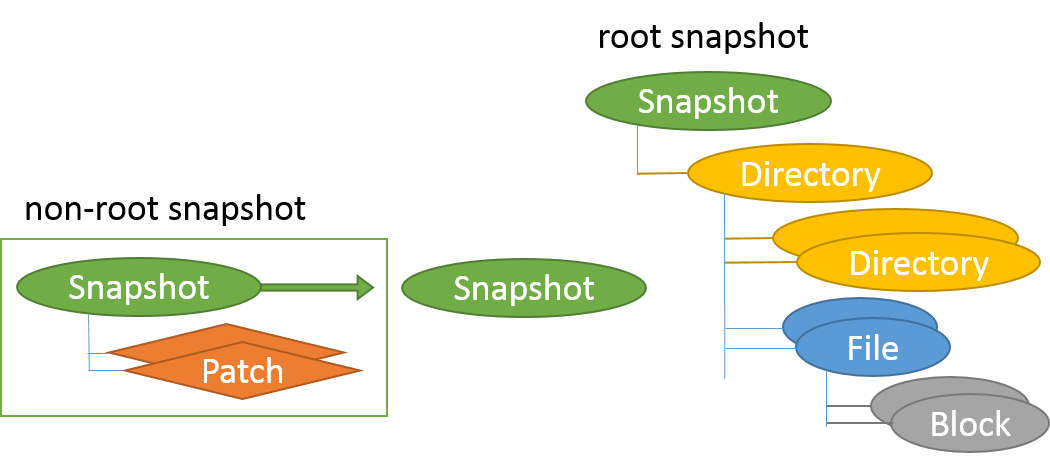
\includegraphics[width=0.75\textwidth]{Chapter-4/figs/fig12.png}
\caption{Root Snapshot and Non-root Snapshot}
\label{fig:root_and_nonroot}
\end{figure}

    A patch object reflects a single or a series of modification to a single node. The node can be either file node or one node. The patch object references a pair of file nodes or directory nodes. The two nodes referred are the target node (original version) and its replacement (changed version).

    \fref{fig:patches} demonstrates the way the patch systemworks. Snapshot 1 and 2 demonstrates how a directory changes between snapshots. The directory that is represented by node $d_2$ in snapshot 2 is now replaced by directory node $d_1$ in snapshot 1. In snapshot 2, the directory has a new subdirectory but the file under that directory remains unchanged. Hence the target node (node $d_2$) and replacement node (node $d_1$) have a reference to the same file node but the target node $d_2$ has one more reference to a directory node. In the example of snapshot ($a$) and snapshot ($b$), a file changes in both snapshot, its original version is $f_1$, the intermedia version in snapshot ($b$) is $f_2$ and final version is $f_3$ in snapshot ($a$). In snapshot $\alpha$ and snapshot $\beta$, file $f_3$ is replaced by $f_2$ in snapshot ($\beta$) and replaced by $f_1$ in snapshot ($\alpha$).  

\begin{figure}[t]
\centering
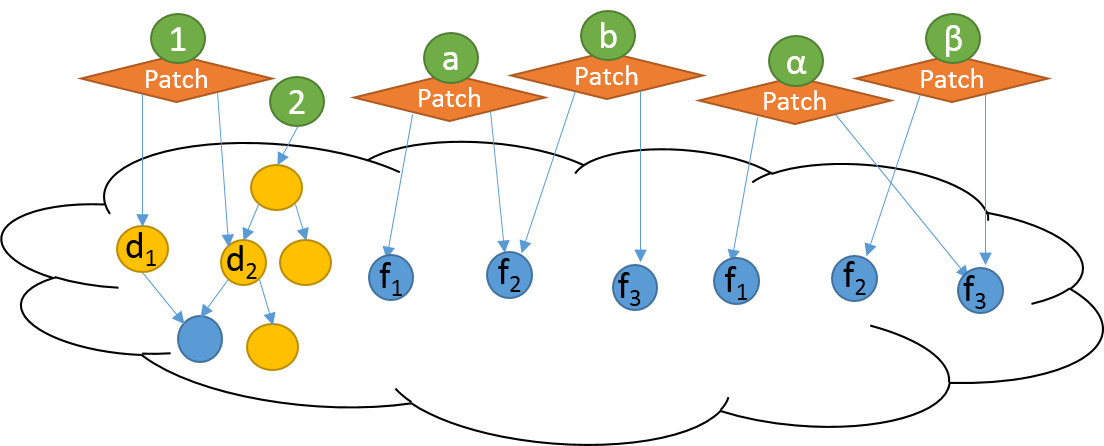
\includegraphics[width=0.75\textwidth]{Chapter-4/figs/fig14.png}
\caption{The Principle of Patches}
\label{fig:patches}
\end{figure}

\section{Snapshot Related Operations}

    Operations in snapshot system involves read the content in a snapshot and make changes to (or write) a writeable snapshot. Make changes to the current view of the file system also involves snapshot write operation as the current view of the file system is also treated as a snapshot in Kabi file system.

\subsection{Read Operations}

    When reading a file or a directory in the referencing snapshot, the file system must to do a large number of lookup in patch lists to ensure that the file system is referring to the correct version of the node. For instance, in \fref{fig:read_patches} , to read the file ``/a/d.txt'' in snapshot 1 shown in figure below, the file system will first read in ``/'' directory in head snapshot which is node 3. Then it transverses all involved snapshots (1 and 2) to see if there's a patch whose target node is node 3. Since no such patch is available, this means node 3 is the ``/'' directory node of all snapshot node (1, 2 and 3). Then the file system will look for “a” directory under node 3 and corresponding patches. In this example, there is a directory (node 9) with display name “a” under node 3 but there is also a patch to node 9 in snapshot 2. That means node 5 is the ``/a'' directory node of snapshot 0 while node 6 is the directory node for snapshot 1 and snapshot 2. Follow the same procedure, we will find node 8 is the ``/a/d.txt'' node in snapshot 2 but for snapshot 1 ``/a/d.txt'' represented by node 6.

\begin{figure}[t]
\centering
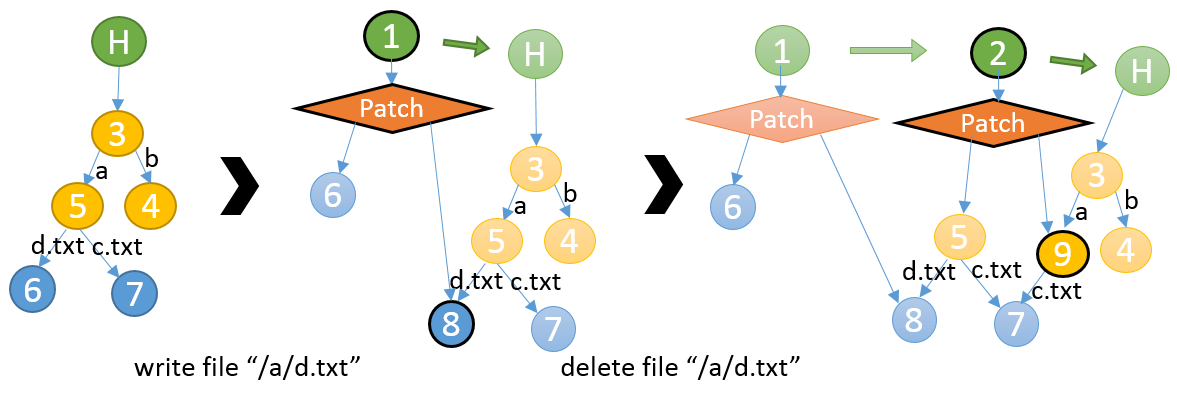
\includegraphics[width=0.5\textwidth]{Chapter-4/figs/fig18.png}
\caption{Read a snapshot}
\label{fig:read_patches}
\end{figure}

    As one can see, read operations rely on the patch lookup operation. To avoid query and traverse all involved snapshot and patch objects on every read operation, a local patch list is built and stored as hashtable in memory when a referencing snapshot node is mounted. The local patch list combines all patches that may be used for a node lookup. In the example shown in \fref{fig:combine_patch_list}, when mounting snapshot 3, a local patch list that contains all effective patches in snapshot 3 and 2 is created.

\begin{figure}[t]
\centering
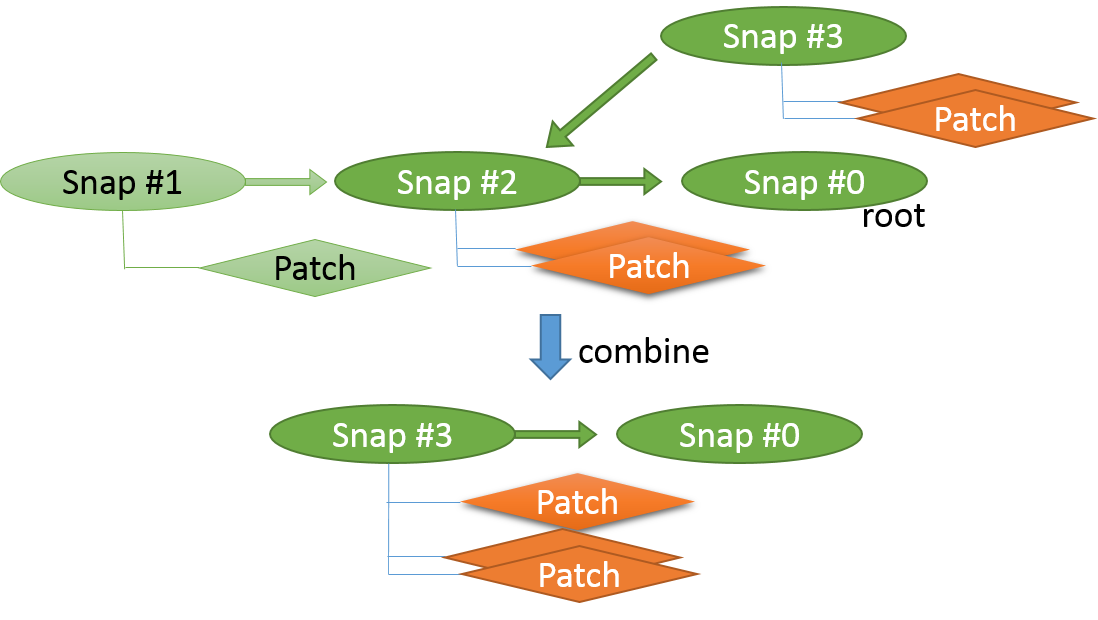
\includegraphics[width=0.8\textwidth]{Chapter-4/figs/fig15.png}
\caption{Combine Patch Lists}
\label{fig:combine_patch_list}
\end{figure}

    Not all patches in patch lists will be combined into a local patch list. Because patches are come from different patch lists, when they combine together some patches are mergeable and some are ineffective. For instance, in \fref{fig:merge} snapshot (a) and (b) the replacement node $f_2$ of a patch is also the target node of another patch, these two patch object can be merged into one local patch. Another example is snapshot ($\alpha$) and ($\beta$), the two patch shown in the figure have the same target node $f_3$. When snapshot ($\alpha$) is mounted, the patch in snapshot ($\beta$) will become ineffective and will not be read in.

\begin{figure}[t]
\centering
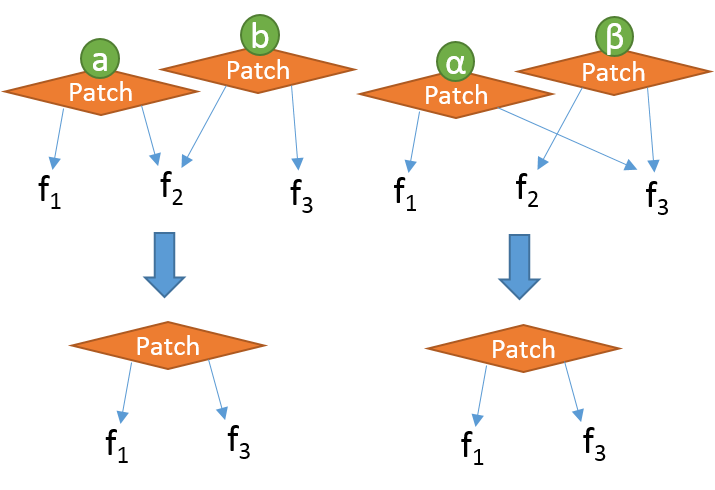
\includegraphics[width=0.7\textwidth]{Chapter-4/figs/fig19.png}
\caption{Merge Patches (Local)}
\label{fig:merge}
\end{figure}

\subsection{Write Operations}

    In both copy-on-write snapshot system or redirect IO snapshot system, a file system entity (block, file, directory) may be referenced one or more times. Referencer could be snapshots or the ``current'' view of the file system. If an entity is referenced only once, write operation to that entity will be straight forward. This is a write operation within a snapshot. On the other hand, when an entity is referenced more than once, the snapshot system usually need special treatment to the write operation. Otherwise a direct in-place write will affect all referencer. In the snapshot system, we focus on the later case. If not otherwise specified, ``write operation'' in this section refers to those write calls whose target entities has been referenced more than once.

	\fref{fig:create_snapshots} briefly demonstrates how patch object and snapshots work with write operations. This example has 3 snapshots. Node 0 is the head snapshot node representing the current status of the main branch. Snapshot node 2 represents the initial status and node 1 is the intermediate status of main branch. Initially, the file system contains three directory ``/'', ``/a'', ``/b'' and two files ``/a/c.txt'', ``/a/d.txt''. In between the initial snapshot and the next snapshot, file ``/a/d.txt'' was overwritten so its representing node is changed by a patch. After snapshot 2 is taken, the file ``/a/d.txt'' was deleted. A new patch is attached to snapshot 2 to reflect this change.

\begin{figure}[t]
\centering
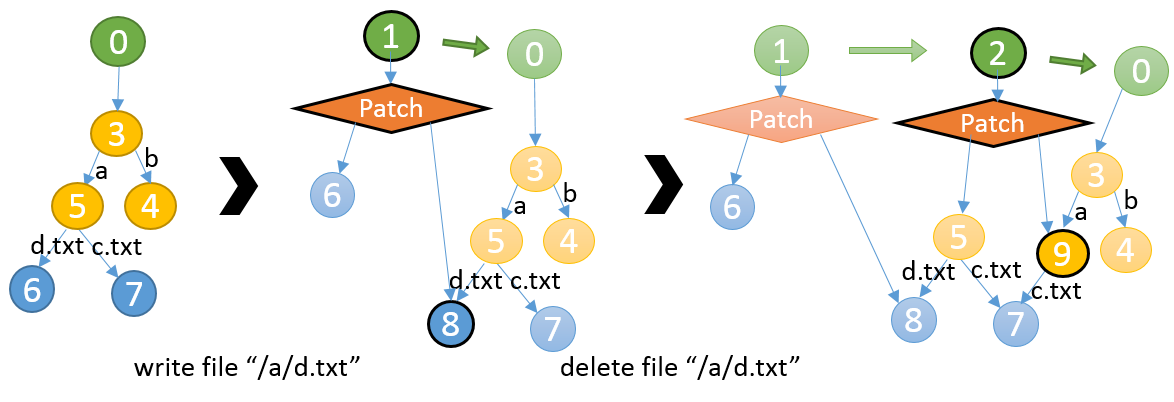
\includegraphics[width=0.95\textwidth]{Chapter-4/figs/fig26.png}
\caption{Example: Create Snapshots}
\label{fig:create_snapshots}
\end{figure}

    \fref{fig:take_snapshot_root} and \fref{fig:take_snapshot_nonroot} shows how to take snapshots on the main branch and side branchs.

    In order to take a new snapshot on the main branch, the file system will create a new snapshot node in between the head snapshot and its adjacent snapshot node. This newly created snapshots will have an empty patch list referencing the head snapshot. This new snapshot node will represent the status of this branch at the time it is created. The current state of the main branch is still the head snapshot.

\begin{figure}[t]
\centering
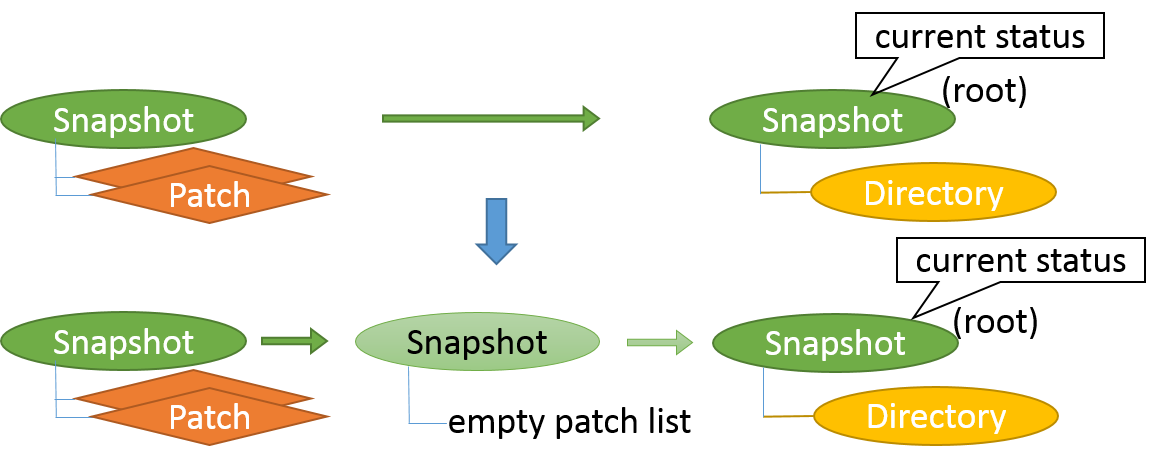
\includegraphics[width=0.8\textwidth]{Chapter-4/figs/fig20.png}
\caption{Take Snapshots on Main Branch}
\label{fig:take_snapshot_root}
\end{figure}
    
	To take a snapshot on a side branch, the file system will create a new snapshot node attached to the end of the side branch. The newly created snapshot node will reference the latest snapshot on this branch and have an empty patch list. After attaching to the branch, this snapshot will become the current status of this branch.

\begin{figure}[t]
\centering
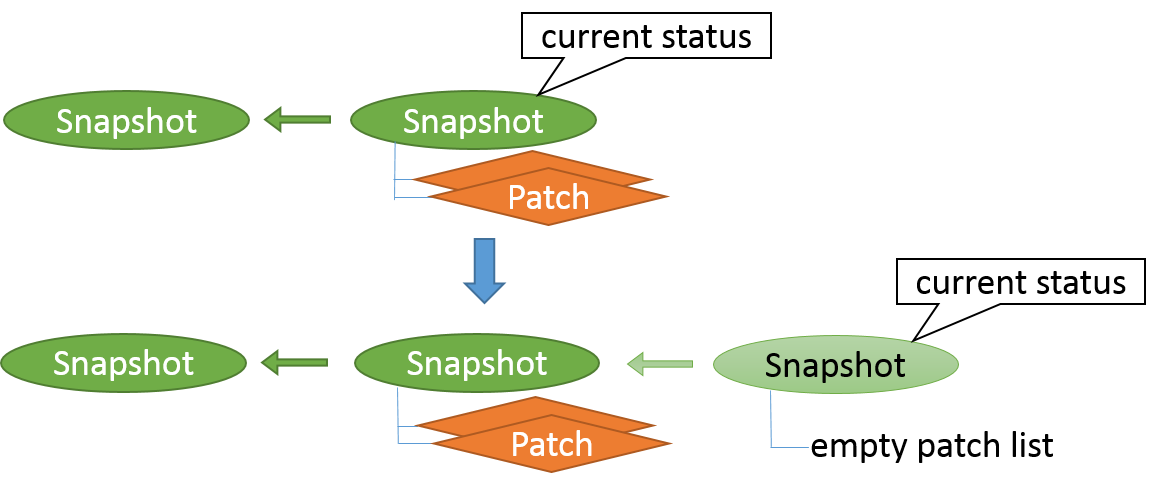
\includegraphics[width=0.8\textwidth]{Chapter-4/figs/fig21.png}
\caption{Take Snapshots on Side Branch}
\label{fig:take_snapshot_nonroot}
\end{figure}
    
    When writing a leaf referencing snapshot, the Kabi File System will submit new patches to that referencing snapshot to reflect the change. In the first example shown in \fref{fig:write_snapshot_node}, the file system is writing the head snapshot in main branch, replacing node X with its newer version Y. Node Y will replace node X directly in the head snapshot. In order to keep its previous version X in snapshot 2, a ``reverse'' patch object (Y-to-X) will be submitted to revert node Y back to its original version X. In this way, the head snapshot will have the new version Y while all other snapshots keep the old version X. In the second example, the file system is trying to replace node X with its new version Y in snapshot 3. Compared to the first example, the file system now can simply submit a X-to-Y patch to snapshot 3. In the third example, we demonstrate a walk around to writing an internal snapshot node by creating a branch based on that internal node and write to that branch.

\begin{figure}[t]
\centering
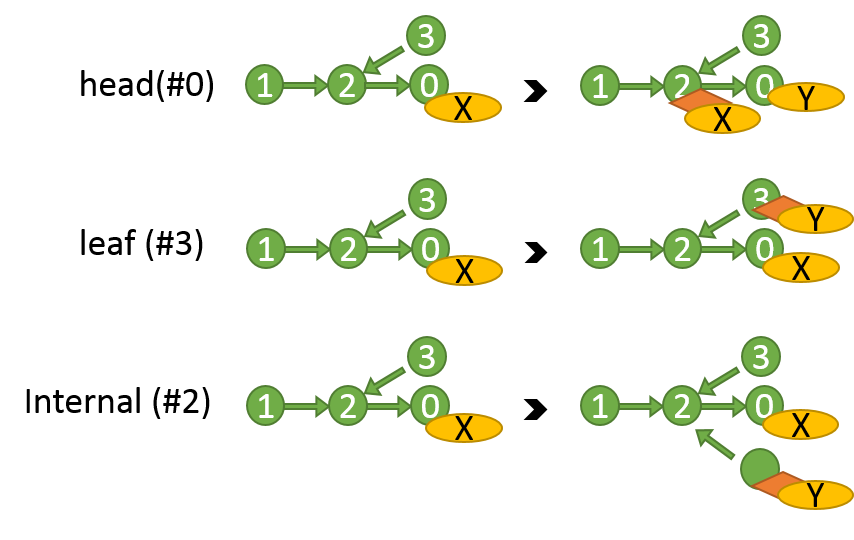
\includegraphics[width=0.7\textwidth]{Chapter-4/figs/fig17.png}
\caption{Write a Snapshot Node}
\label{fig:write_snapshot_node}
\end{figure}

    To create a branch based on the head snapshot, it is recommended to create a dummy snapshot first and then fork from that dummy node rather than branching the head snapshot directly. This is because a write operation to head snapshot will submit patches to all snapshot nodes connected to head snapshot node. Hence we wish to limit the number of snapshots connected to the head snapshot. If we fork the head snapshot directly then there will be multiple snapshot nodes connected on to the head snapshot node. \fref{fig:dummy_node} demonstrates this issue:

\begin{figure}[t]
\centering
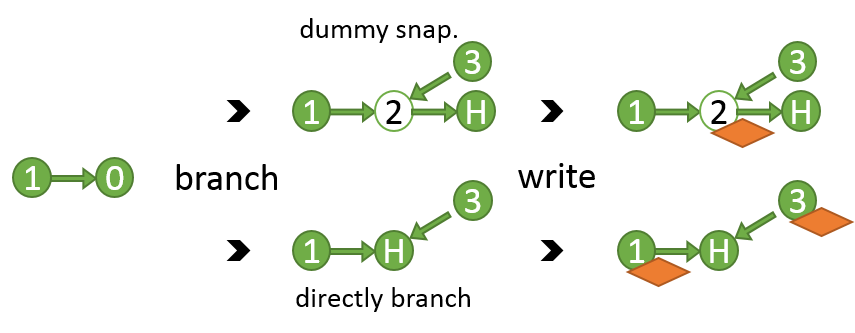
\includegraphics[width=0.8\textwidth]{Chapter-4/figs/fig16.png}
\caption{Branching Root Snapshot Node Directly}
\label{fig:dummy_node}
\end{figure}

	Generally, within a snapshot, each node (file or directory) should have no more than one patch associated with it. For example, a patch replacing node 0 with node 1 and a patch replacing node 1 with node 2 can be merged into one patch. This happens when a node is modified multiple times. For time and space efficiency, it is better to merge them into one patch.
	
\section{Enhancing Copy-on-Write and Deduplication}

	The copy-on-write strategy and file system deduplication improve space efficiency of the file system. File system deduplication finds and eliminates duplicated blocks and files while the classical copy-on-write strategy eliminates unnecessary copy of an unchanged block to snapshots.

\subsection{Motivation}

    A classical copy-on-write snapshot system applies copy-on-write at block level. As shown in \fref{fig:classic_cow}, unchanged blocks will not be copied to the snapshot.

\begin{figure}[t]
\centering
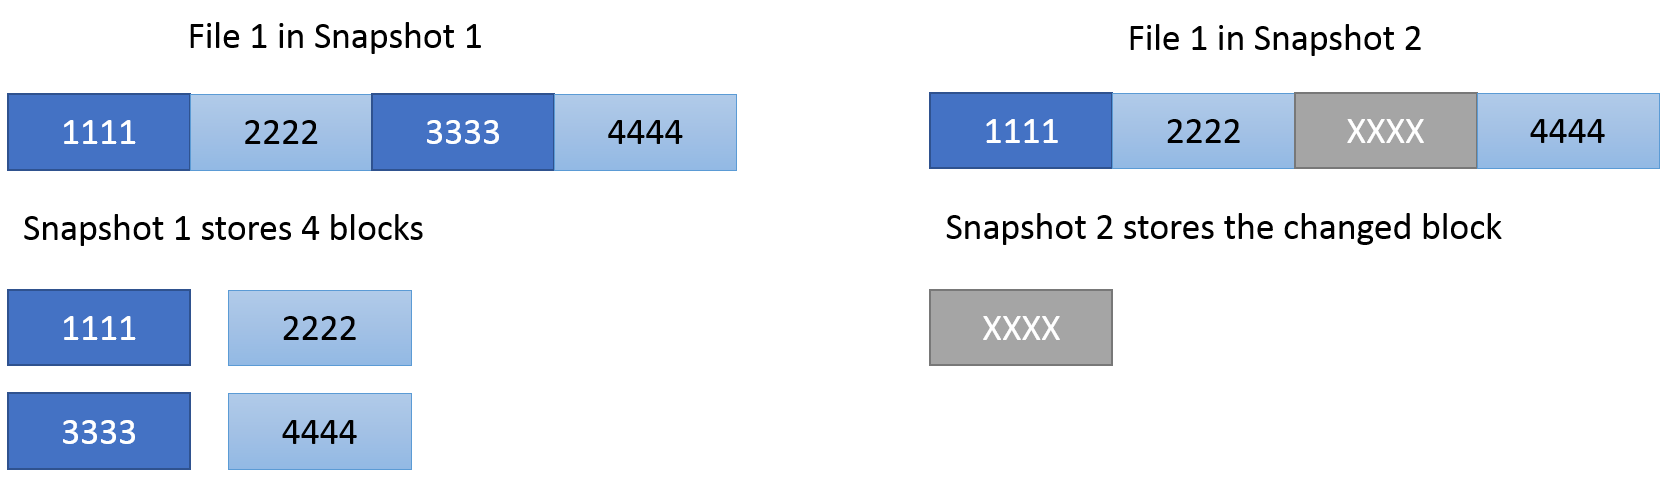
\includegraphics[width=0.8\textwidth]{Chapter-4/figs/fig4.png}
\caption{Classic Copy-on-Write}
\label{fig:classic_cow}
\end{figure}

    However, in reality it is not always an ideal solution. In many use cases like insertion or deletion, a write operation only affects a few bytes instead of a whole block. But a classic file system will rewrite all successor blocks in these scenarios. A classical snapshot system will make a copy of all successor blocks despite the fact that only very few bytes is changed. The following \fref{fig:issue_classic_cow} addresses this issue. In this example, a byte is inserted into the file at offset 8. In classical copy-on-write snapshot system, 2 successor blocks are treated as changed blocks and will be copied. However, actually, the data in those blocks did not change. They only moved one byte forward. In the figure we also demonstrates a potentially better approach.

\begin{figure}[t]
\centering
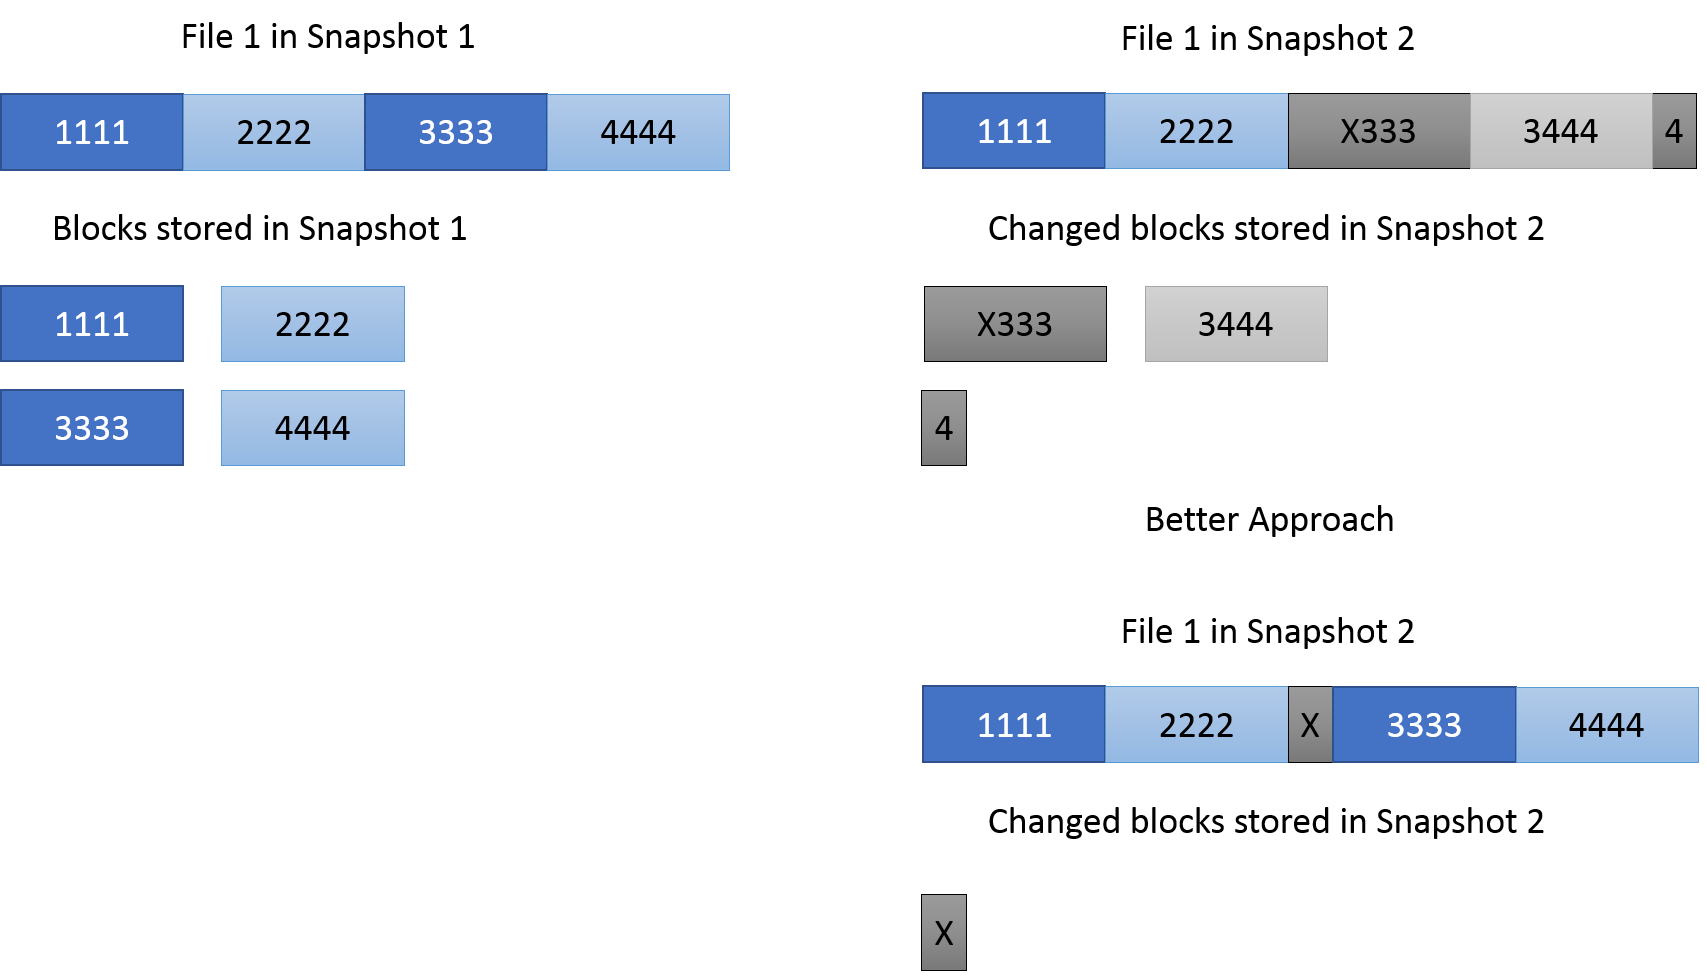
\includegraphics[width=0.8\textwidth]{Chapter-4/figs/fig5.png}
\caption{Issue in Classic Copy-on-Write}
\label{fig:issue_classic_cow}
\end{figure}
 
    To solve this problem, we have to let the file system be aware of the true intention of the end user. This is not straightforward because the POSIX standard uses only one file system call to handle all kinds of modification to a file. The only function of this file system call is to rewrite a part of a file.
    
    If the user program intend to insert a byte right in the middle of the file, the file system will receive a set of write calls to rewrite all later blocks in order to move original data 1 byte forward. The same behavior can also be observed when user program trying to rewrite the later half of the file. It is difficult for the file system to distinguish these two scenario. Access patterns can be used to guess the intention of an operation (i.e. an insertion usually results in a truncate call followed by a series of write() calls), but it is not an ideal solution as it depend on how the user program will behave. Therefore our major challenge is to identify the true intention of an write operation, whether should be an insertion or a complete rewrite.

    In this chapter we will show how to accomplish this goal by using the rsync algorithm.

\begin{figure}[t]
\centering
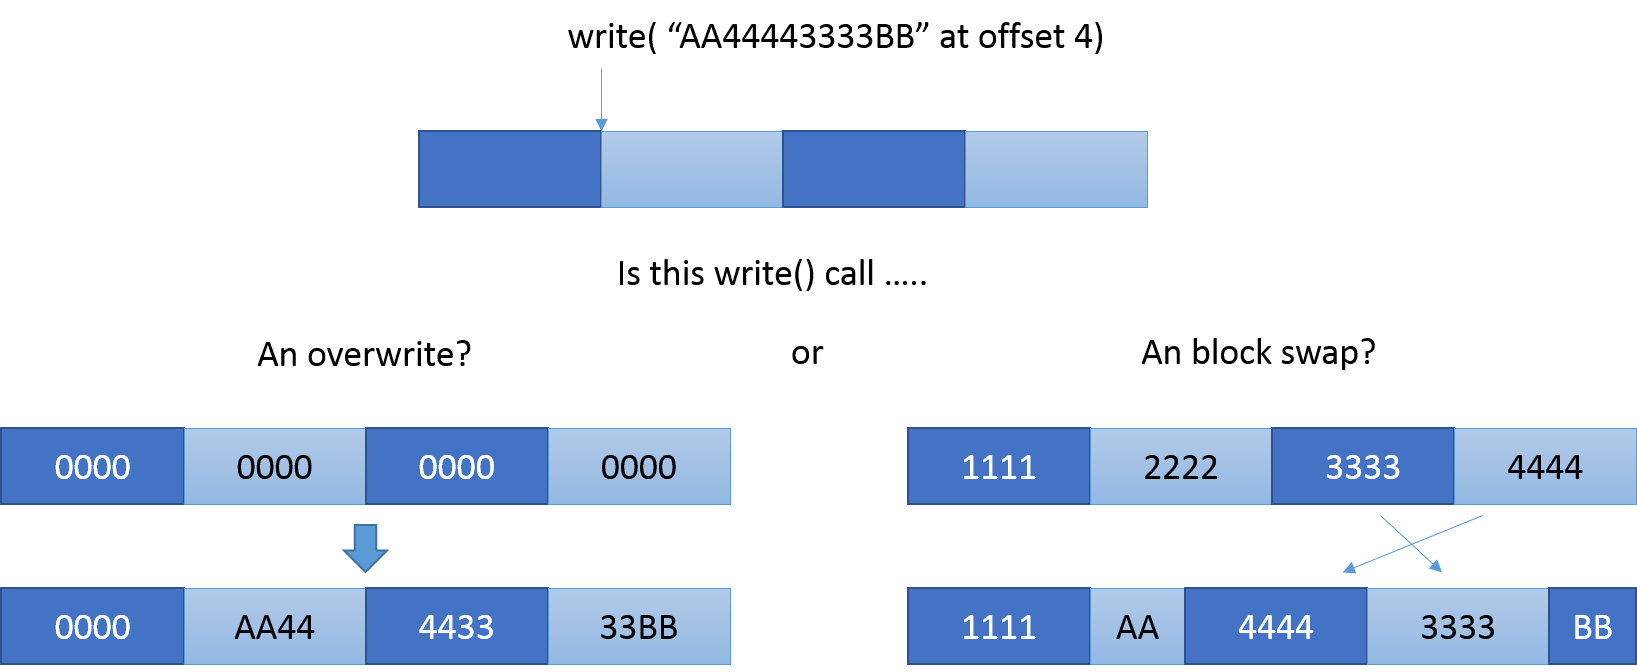
\includegraphics[width=0.8\textwidth]{Chapter-4/figs/fig6.png}
\caption{Identify the intention of write operations}
\label{fig:write_intention}
\end{figure}

\subsection{The rsync algorithm}

    As discussed in the previous section, in order to identify duplication in a better way, we need to have a mechanism to compare the data to be written into the file and the original data. 
    
    The rsync algorithm is originally designed for the efficient update of data over a high latency and low bandwidth link. Compared to brute force search and string search algorithms, rsync algorithm is much faster in practice and requires less data exchange between the remote server and local machine. These features make it suitable for a distributed file system. Because both time consuming file system and a high bandwidth consumption file system will become a bottleneck in the operating system.

    The basic flow of the rsync algorithm is to split the remote file into blocks of length $S$, calculate their rolling checksum and then send their them to the local machine. The local machine will search through local file to find all blocks of length $S$ bytes (at any offset, not just multiples of $S$) that matches the received rolling checksum. This can be done in a single pass very quickly since the rolling checksum only requires $O(1)$ time to compute checksum at offset k given the checksum at offset $k-1$.

\subsection{Enhancing the space efficiency}

    The Kabi File System uses the rsync algorithm to enhance the space efficiency of snapshots. It assumes that in most cases two different versions of the same file will share part of their data.

    In the Kabi File System, a section object in a file node contains not only the reference to the corresponding block, but also contains the rolling checksum of the block data. Before flushing the write buffer, the local machine will calculate the rolling checksum of data block at all possible offsets. The file system will compare these rolling checksums with those fetched from remote. If a match is found, the file system will then double check their SHA-1 hash to confirm that it is indeed a duplication.
    
    Once all data blocks have been examined, the local machine will send the ID of duplicated blocks and all remaining data back to the remote server.


\begin{figure}[t]
\centering
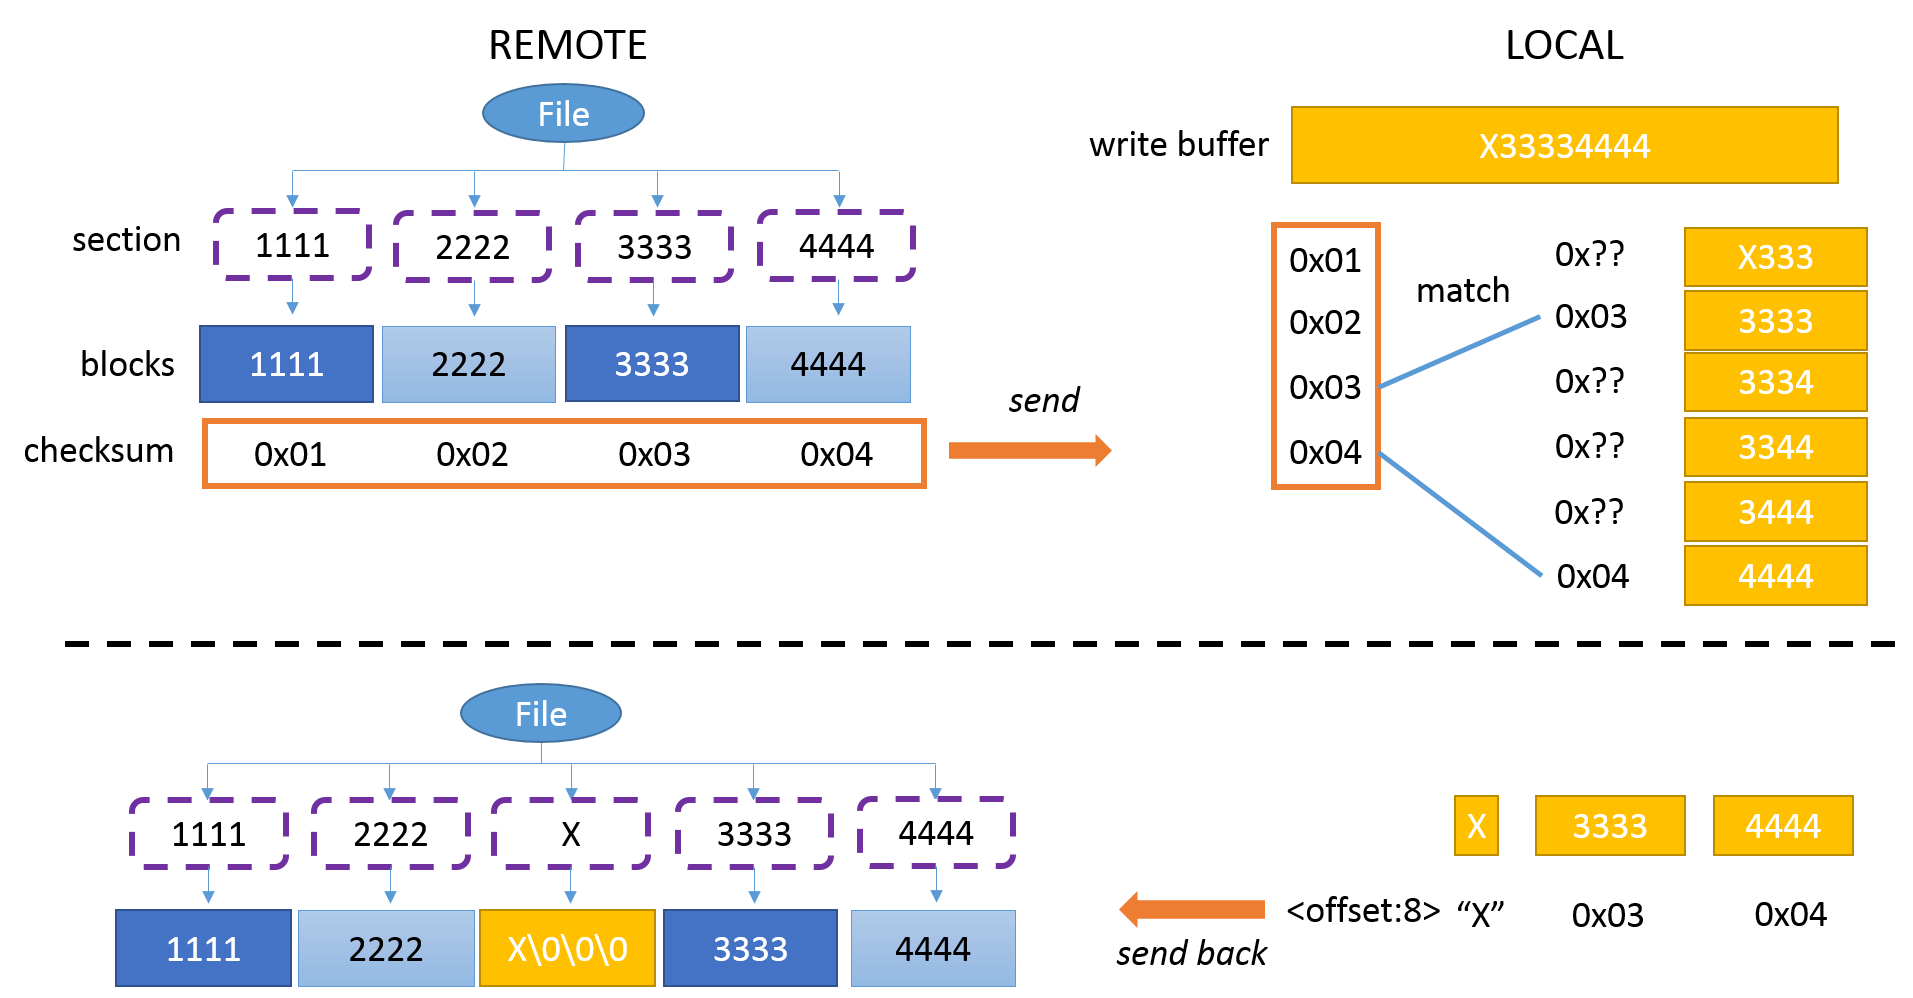
\includegraphics[width=0.9\textwidth]{Chapter-4/figs/fig25.png}
\caption{Using rsync to find unchanged blocks}
\label{fig:rsync}
\end{figure}

    During this process, the computational overhead is only the calculation and matching of rolling checksums. An important property of rolling checksum algorithm is that successive values can be computed in $O(1)$ time, thus ensuring that all rolling checksums can be calculated in $O(n)$ time. In contrast the benefits are a significant decrease in network flow and remote storage when there is duplicate data in buffer.

\section{Conclusion}

   In this chapter, we present the basic idea of this snapshot system and discuess some implementation details of the snapshot subsystem in Kabi File System. We demonstrated our efforts to make the snapshot system efficient in space usage. We also introduced the rsync algorithm to improve the snapshot system and the network performance.
